\documentclass{article}
\usepackage{amsmath}
\usepackage{amssymb}
\usepackage{amsfonts}
\usepackage{titling}
\usepackage{graphicx}

\providecommand{\abs}[1]{\left\vert#1\right\vert}
\let\vec\mathbf

\title{\textbf{Construction}}
\date{}

\begin{document}

\maketitle

\begin{enumerate}
	\item In the given figure, $XZ$ is parallel to $BC$. $AZ$ = 3cm, $ZC$ = 2cm, $BM$ = 3cm and $MC$ = 5cm. Find the length of $XY$.
		\begin{figure}[h!]
			\centering
			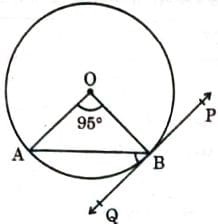
\includegraphics [width=\columnwidth] {figs/fig1.jpg}
			\caption{Isosceles Triangle}
			\label{fig:fig1.jpg}
		\end{figure}

	\item In the given figure, $DE$ $||$ $BC$. If $AD$ = 2units, $DB$ = $AE$ = 3units and $EC$ = $x$units, then find the value of $x$ is:\\

		\begin{figure}[h!]
			\centering
			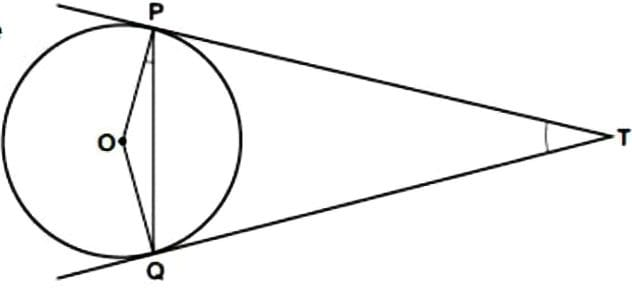
\includegraphics [width=\columnwidth] {figs/fig2.jpg}
			\caption{Right Angle Triangle}
			\label{fig:fig2.jpg}
		\end{figure}

			\begin{enumerate}
				\item 2
				\item 3
				\item 5
				\item $\frac{9}{2}$
			\end{enumerate}

		\newpage

	\item In the given figure, $\Delta ABC$ and $\Delta DBC$ are on te same base $BC$. If $AD$ intersects $BC$ at $\vec{O}$, prove that $\frac { ar(\Delta ABC)}{ar (\Delta DBC)}$ = $\frac{AO}{DO}$.

		\begin{figure}[h!]
			\centering
			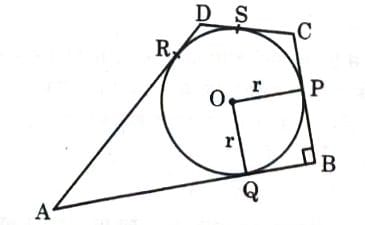
\includegraphics [width=\columnwidth] {figs/fig3.jpg}
			\caption{Triangles with same base}
			\label{fig:fig3.jpg}
		\end{figure}
\pagebreak

\title{\textbf{Linear}}
\date{}
\maketitle

	\item \textbf{Assertion (A):} Point $\vec{P}$(0,2) is the point of intersection of $y-axis$ with  the line $3x+2y=4$.\\
		\textbf{Reason (R):} The distance of point $\vec{P}$(0,2) from $x-axis$ is 2 units.


	\item If the pair of equations $3x-y+8=0$ and $6x-ry+16=0$ represent coincident lines, then the value of \text{'$r$'} is:

		\begin{enumerate}
			\item $-\frac{1}{2}$
			\item $\frac{1}{2}$
			\item -2
			\item 2
		\end{enumerate}

	\item The of linear equations $2x=5y+6$ and $15y=6x-18$ represents two lines which are:

			\begin{enumerate}
				\item intersecting
				\item parallel
				\item coincident
				\item either intersecting or parallel
			\end{enumerate}

		\item Find the equations of the diagonals of the parallelogram $\vec{PQRS}$ whose vertices are $\vec{P}$(4,2,-6), $\vec{Q}$(5,-3,1), $\vec{R}$(12,4,5) and $\vec{S}$(11,9,-2). Use these equations to find the point of intersection of diagonals.

	\item A line $l$ passes through point (-1,3,-2) and is perpendicular to both the lines $\frac {x}{1}=\frac{y}{2}=\frac{z}{3}$ and $\frac {x+2}{-3}=\frac{y-1}{2}=\frac{z+1}{5}$. Find the ctor equation of the line $l$. Hence, obtain its distance from origin.

\end{enumerate}
\end{document}
